\documentclass{article}

% Packages
\usepackage{amsmath, amssymb}   % math formatting & symbols
\usepackage{graphicx}           % insert graphics
\usepackage{listings}
%\usepackage{eulervm, bookman}   % fonts for math & symbols
\usepackage{fullpage}          % fullpage margins

\lstset{language=Matlab,
    basicstyle=\scriptsize\ttfamily,
    stringstyle=\ttfamily,
    showstringspaces=false,
    breaklines=true,
    frameround=ffff,
    frame=single,
}

\begin{document}
% Title 
\title{Math 104A: Homework 5}
\author{Raghav Thirumulu, Perm 3499720 \\ \texttt{rrajuthirumulu@umail.ucsb.edu}}
\maketitle

\begin{enumerate}
    \item % 1 
        \begin{enumerate}
            \item 
            Assuming that $q \in P_n $, we can say that $q$ is a polynomial of degree at most n. In other words, we can write
            \begin{align*}
                q = \sum_{j=0}^{n} b_j\psi_j
            \end{align*}
            Using properties of inner products and the given equations, we can write the following:
            \begin{align}
            <f-P_n,q> &= <f,q> - <P_n,q> \\
                      &= <f,\sum_{j=0}^{n} b_j\psi_j> - <\sum_{j=0}^{n} a_j\psi_j, \sum_{j=0}^{n} b_j\psi_j> \\
                      &= \sum_{j=0}^{n} b_j <f,\psi_j> - \sum_{j=0}^{n} a_jb_j <\psi_j,\psi_j>
            \end{align}
            Rewriting the given equation, we obtain:
            \begin{align*}
            <f,\psi_j> = a_j<\psi_j,\psi_j>
            \end{align*}
            So equation (3) simplifies to 
            \begin{align*}
            <f-P_n,q> &= \sum_{j=0}^{n} a_jb_j <\psi_j,\psi_j> - \sum_{j=0}^{n} a_jb_j <\psi_j,\psi_j> \\
                      &= 0
            \end{align*}
            Hence the error term $ f - P_n $ is orthogonal to $q$ or any polynomial of degree $n$.
            \item
            We know from part (a) that $ f - P_n $ is orthogonal to any polynomial from $P_n$, so we can write 
            \begin{align*}
                P_n + (f-P_n) = f
            \end{align*}
            We can then deduce that $f$ is the sum of two orthogonal vectors. Let $U$ and $V$ denote the subspaces, containing each of these orthogonal vectors, respectively, as follows:
            \begin{align*}
                U &= P_n \\
                V &= f-P_n
            \end{align*}
            We can say there is an orthogonal projection from the space $P_n$ onto the two subspaces containing $U$ and $V$. The equations are shown as follows:
            \begin{align*}
                proj_U(f-P_n) &= proj_U(f) - proj_U(P_n) \\
                              &= P_n - P_n = 0
            \end{align*}
            We then can write:
            \begin{align*}
                proj_U(P_n) + proj_U(f-P_n) &= proj_U(P_n) + 0 \\
                                            &= proj_U(P_n)
            \end{align*}
        \end{enumerate}
    \item % 2
        \begin{enumerate}
            \item
            We find the Legendre polynomials using the following formula:
            \begin{align*}
                P_0(x) &= 1 \\
                P_n(x) &= \frac{1}{n!2^n}\frac{d^n}{dx^n}(x^2-1)^n
            \end{align*}
            Therefore, the first four Legendre polynomials are:
            \begin{align*}
                P_0(x) &= 1 \\
                P_1(x) &= x \\
                P_2(x) &= \frac{1}{2}(3x^2-1) \\
                P_3(x) &= \frac{1}{2}(5x^3-3x)
            \end{align*}
            \item
            We use the following formula to find the least square approximation: 
            \begin{center}
                $ l_n(x) = \sum_{j=0}^{n} \frac{<f,P_j>}{<P_j,P_j>}P_j(x) $
            \end{center}
            where each $ P(x)$ is a Legendre polynomial. Therefore,
            \begin{center}
                $ l_n(x) = \sum_{j=0}^{n} \beta_jP_j(x) $ where $ \beta_j = \frac{<f,P_j>}{<P_j,P_j>}$
            \end{center}
            So
            \begin{align*}
                \beta_0 &= \frac{<f,P_0>}{<P_0,P_0>} \\
                        &= \frac{\int_{-1}^{1}(1)(e^x)dx}{\int_{-1}^{1}(1)(1)dx} \\
                        &= \frac{1}{2}(e-1/e) \\
                        &= 1.1752 \\ \\
                \beta_1 &= \frac{<f,P_1>}{<P_1,P_1>} \\
                        &= \frac{\int_{-1}^{1}(x)(e^x)dx}{\int_{-1}^{1}(x)(x)dx} \\
                        &= 1.1037 \\ \\
                \beta_2 &= \frac{<f,P_2>}{<P_2,P_2>} \\
                        &= \frac{\frac{1}{2}\int_{-1}^{1}(3x^2-1)(e^x)dx}{\frac{1}{4}\int_{-1}^{1}(3x^2-1)^2dx} \\
                        &= 0.3564 \\ \\
                \beta_3 &= \frac{<f,P_3>}{<P_3,P_3>} \\
                        &= \frac{\frac{1}{2}\int_{-1}^{1}(5x^3-3x)(e^x)dx}{\frac{1}{4}\int_{-1}^{1}(5x^3-3x)^2dx} \\
                        &= 0.0803
            \end{align*}
            So
            \begin{align*}
                l_1(x) &= \beta_0P_0(x) + \beta_1P_1(x) \\
                       &= 1.1752(1) + 1.1037(x) \\
                       &= 1.1752 + 1.1037x \\ \\
                l_2(x) &= \beta_0P_0(x) + \beta_1P_1(x) + \beta_2P_2(x) \\
                       &= 1.1752(1) + 1.1037(x) + 0.3664(0.5)(3x^2-1) \\ \\
                l_3(x) &= \beta_0P_0(x) + \beta_1P_1(x) + \beta_2P_2(x) + \beta_3P_3(x) \\
                       &= 1.1752(1) + 1.1037(x) + 0.3664(0.5)(3x^2-1) + 0.0803(0.5)(5x^3-3x) \\
                       &= 0.9968 + 0.9832x + 0.5340x^2 + 0.2008x^3
            \end{align*}
            \item
            Let $ a_0 + a_1x + a_2x^2 + a_3x^3 + a_4x^4$ be the least square approximation for $ f(x)=x^3$ on [-1,1]. \\
            
            Using the least square approximation method, we obtain the following system of equations (not shown because the scratch work is very long):
            \begin{align}
                30a_0 + 10a_2 + 6a_4 &= 0 \\
                10a_1 + 6a_3 &= 6 \\
                70a_0 + 42a_2 + 30a_4 &= 0 \\
                14a_1 + 10a_3 &= 10 \\
                126a_0 + 90a_2 + 70a_4 &= 0
            \end{align}
            
            Combining equations (5) and (7) we obtain $ a_3 = 1$. Solving for the other constants we get $ a_0 = a_1 = a_2 = a_4 = 0$. Therefore, the least square approximation is $x^3$. This is because we are attempting to approximate a polynomial of degree 3 with a 4 degree approximation. So we get an accurate result. 
        \end{enumerate}
    \item % 3
        The first 5 Chebyshev polynomials are given as follows: 
        \begin{align*}
        T_0(x) &= 1 \\
        T_1(x) &= x \\
        T_2(x) &= 2x^2-1 \\
        T_3(x) &= 4x^3-3x \\
        T_4(x) &= 8x^4-8x^2+1 \\
        \end{align*}
        Using the following formulas:
        \begin{align*}
            \widetilde{T}_0(x) &= 1 \\
            \widetilde{T}_n(x) &= \frac{1}{2^{n-1}}T_n(x)
        \end{align*}
        we obtain the monic Chebyshev polynomials as follows:
        \begin{align*}
        \widetilde{T}_0(x) &= 1 \\
        \widetilde{T}_1(x) &= x \\
        \widetilde{T}_2(x) &= x^2-\frac{1}{2} \\
        \widetilde{T}_3(x) &= x^3-\frac{3}{4}x \\
        \widetilde{T}_4(x) &= x^4-x^2+\frac{1}{8} \\
        \end{align*}
        Here is the code for plotting the functions above, along with the figure:
        \begin{lstlisting}
        % Computer code for plotting Monic Chebyshev polynomials
        %
        % Input: No arguments are necessary for running this function
        % Output: A plot of T0(x), T1(x), T2(x), T3(x), T4(x)
        %
        % Author: Raghav Thirumulu, Perm 3499720
        % Date:   07/24/2018

        x=-1:.01:1;

        T0 = x.^0;
        T1 = x;
        T2 = (x.^2) - 0.5;
        T3 = (x.^3) - (0.75.*x);
        T4 = (x.^4) - (x.^2) + 1/8;

        plot(x,T0,'b'); hold on
        plot(x,T1,'r');
        plot(x,T2,'g');
        plot(x,T3,'m');
        plot(x,T4,'k');
        title('Monic Chebyshev Polynomials');
        axis([-1 1 -1.2 1.2]);
        legend('T_0(x)','T_1(x)','T_2(x)','T_3(x)','T_4(x)');
        xlabel('x');
        ylabel('T(x)'); hold off

        \end{lstlisting}
        \begin{center}
            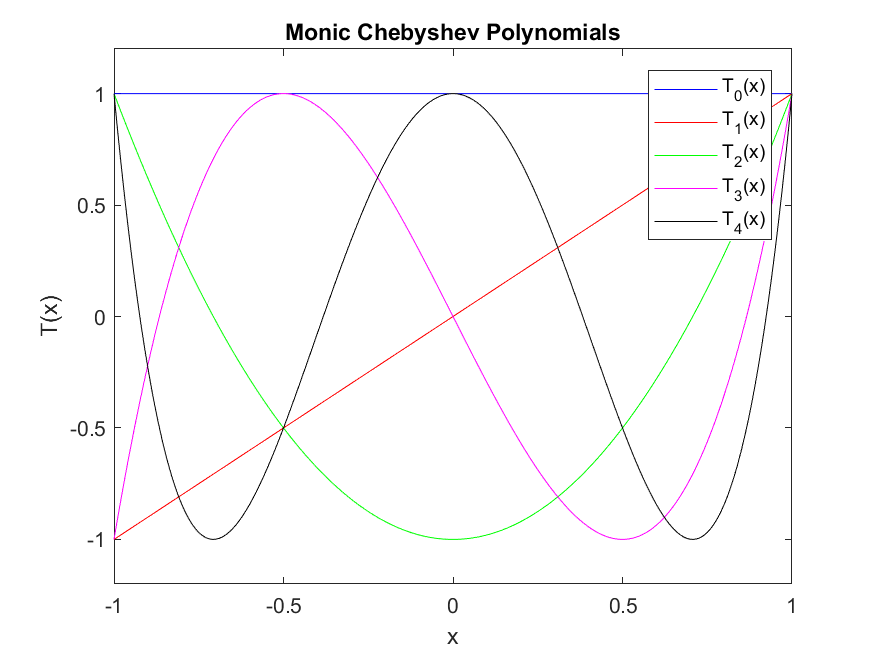
\includegraphics[scale=0.7]{monic.png}
        \end{center}
        
        \item
        \begin{enumerate}
            \item 
            \begin{align*}
                c(t) &= be^{-at} \\
                ln(c(t)) &= ln(be^{-at}) \\
                &= lnb + ln(e^{-at}) \\
                &= lnb - at \\
                &= lnb - 0.1t
            \end{align*}
            We can now set up the equation $y = A + Bt$ when $y=lnc, A=lnb, B=-0.1$. The normal equations are of the form:
            \begin{align}
                \sum{y_i} &= 4A + (\sum{t_i})B \\
                \sum{(t_iy_i)} &= (\sum{t_i})A + (\sum{t_i}^2)B 
            \end{align}
            We must now tabulate the data so we can solve for A and B:\\ \\
            \begin{table}
            \centering
            \begin{tabular}{||c c c c c||} 
            \hline
            t_i & c(t) & t_i^2 & y_i & t_iy_i  \\ [0.5ex] 
            \hline \hline
            1 & 0.91 & 1 & -0.0943 & -0.0943 \\ 
            \hline
            2 & 0.80 & 4 & -0.2231 & -0.4462 \\
            \hline
            3 & 0.76 & 9 & -0.2744 & -0.8232 \\
            \hline
            4 & 0.05 & 16 & -0.4307 & -1.7228 \\
            \hline
            \end{tabular} 
            \end{table}
            \\
            So now we obtain:
            \begin{align*}
                \sum{t_i} &= 10 \\
                \sum{t_i^2} &= 30 \\
                \sum{y_i} &= -1.0225 \\
                \sum{(t_iy_i)} &= -3.0865
            \end{align*}
            Plugging in these values back into the normal equations (9) and (10) gives us $A = 0.0095, B=-0.1$
            So now our equation becomes $c(t) = (e^{0.0095})(e^{-0.1t}) = (1.0095)e^{-0.1t}$. So our initial concentration for $t=0$ is 1.0095
            \item
            Our error term takes the form:
            \begin{align*}
                S^2 &= \sum(y_i-f(t_i))^2 \\
                &= (0.91-0.91343)^2 + (0.8-0.8265)^2 + (0.76-0.7478)^2 + (0.65-0.6766)^2 \\
                &= 0.0015704
            \end{align*}
        \end{enumerate}
\end{enumerate}
\end{document}
